%===================================== CHAP 4 =================================

\chapter{Case Study: The Life Science Building Project}
\begin{figure}[h!]
    \centering
    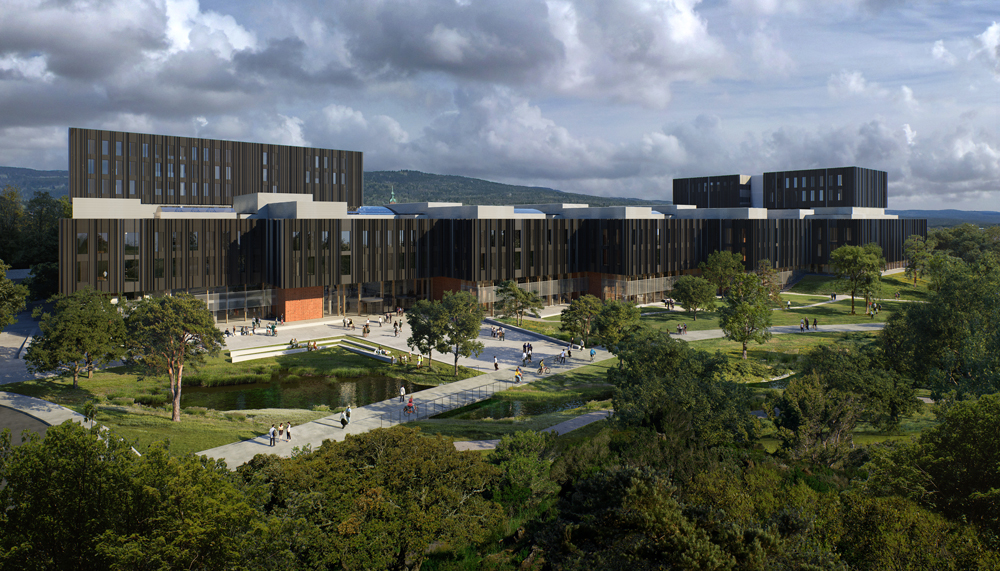
\includegraphics[width=\textwidth]{fig/bygget.jpg}
    \caption{The Life Science Building illustrated exterior (Statsbygg v/Ratio Arkitekter as).}
    \label{fig:illustration}
\end{figure}
\pagebreak
This chapter will, first, introduce the case object, namely the Life Science Building-project. The presentation is an introduction to the project in itself, and the vision and strategies essential for project management. Furthermore, the case study will examine and discuss the findings of the empirical study. Section \ref{sec:case-intro} inherited from the project thesis conducted in the fall of 2019, only upgraded where the information was lacking or inexact.


\section{Introduction of the Life Science Building Project} \label{sec:case-intro} 
The project case will examine the construction of the new life science building of the University of Oslo. When finished, the building will reach a cost of approximately 6,8 million Norwegian Kroner (NOK), and cover 66,700 square meters, with this, becoming the most extensive, detached university building in Norway. Construction owner is the Norwegian Directorate of Public Construction and Property Management (Statsbygg). The construction started on the 8 of February 2019 and is expected to finish in 2024, while the project management of this report started in 2017. The project group, designing the project, however, started their work in 2014.

The manager, Stasbygg, is a significant organization in the Norwegian construction industry. They are on a state mission, which means that they are to realize the politics decided by the government, achieved in architecture, cultural legacy, spatial planning, and environment. 

Each year, Statsbygg constructs about 100 construction projects. Some are more complex than others. The life science Building is one of the more complex. In addition to the construction of new buildings and projects, Statsbygg managing about 600 properties of these 90 outside of Norway. Examples of properties managed by Statsbygg are embassies, royal properties, colleges, and cultural buildings. 

In regards to complexity, the new life science building has to meet several complex requirements: (1) the environmental: The property is to achieve Excellent in the BREEAM NOR classification of sustainable properties; (2) usability: a group of the final users has given their feedback on what they expect from the final building; and (3) technical requirements: The building is to house several faculties, some requires highly technical labs.

\subsection{Project Vision and Strategies} \label{sec:strategy}
The construcionn of the new Life Science Building is, in many ways, a prestige project. Defined in the vision:
\begin{quote}
    \textit{"An even better project"}
\end{quote}
The project is following in the line of previous two large projects running Lean Construction, with Statsbygg as manager. Starting with the Domus Medica construction concluded in 2013. This project was the first Norwegian group applying Lean. This construction was followed by the raising of the new Bergen Academy of Art and Design (BAAD). During these projects, Lean Construction was a significant part of the project management. The first project suffered substantial scope creep, which made the managers take action, applying Lean Design and Systematic Completion \textit{Systematisk Ferdigstillelse} on the BAAD-project. The moves made gave results, and when finished in 2017, the project was by many considered one the most successful (complex) building-constructions completed in Norway.

Based on the the BAAD-project a the \textit{Lean methodology in design and construction}-book \cite{lean_i_praksis} descibing the experience from the project, was made. With the previous history and recomendations from the book, Stasbygg, as a manager, defined five superior strategies in the upcoming LSB-project: 
\begin{enumerate}
    \item The Contract strategy
    \item The Lean strategy
    \item Stretegy of Systematic completion
    \item Digitalization strategy
    \item Logistics strategy
\end{enumerate}
These strategies affect how the project should run and emphasize the focus of the project managers, hopefully leading to a sustainable and productive project. Following are a brief introduction to the different strategies as a context for the case. An holistic view of the strategies in the project are illustrated in figure \ref{fig:strategy}. 

\begin{figure}
    \centering
    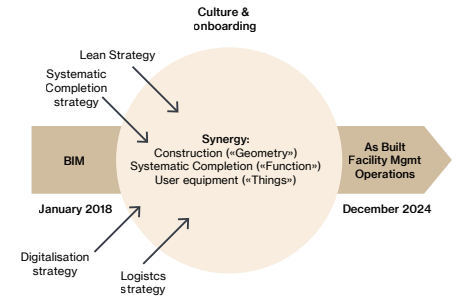
\includegraphics[width=0.8\textwidth]{fig/LVB_strategy.png}
    \caption{A hollistic view of Strategies in the Life Science Building-project.}
    \label{fig:strategy}
\end{figure}

\subsubsection*{The Contract Strategy}
The project has made use of a customized version of the Total Contract, named by Statsbygg as Total Contract with Prior Interaction \textit{(Totalentreprise med forutgående samspill)}. Instead of signing single contracts with each subcontractor, the managers have assembled eight arrangements, each covering different divisions of the project. Hereunder a more Lead Contract type is applied. Figure \ref{fig:project_contracts}displays the eight contract divisions. Responsible for each of the contracts, from management, is either the project manager from construction or technical. Prior Interaction applies to the design phase, where entrepreneurs are involved prior to the job they are to perform. 

The motivation for this model is, first, shielding the contractors from some of the risk running the project. The project is, as mentioned, very intricate in construction, as well as in management. Moreover, getting contractors willing to apply on the project, the managers will take much of the risk. Regarding cooperation the projects adds Lead Contracts. The intention of this is cooperation; besides, sharing a contract has the plan of shared responsibility and incentives for collaboration between subcontractors. Even though there is a lead contractor per division, the hope is that the group of subcontractors should feel shared responsibility. Why not have a shared responsibility,and no leading contractor, one may ask? The answer is partly laws and politics, but moreover for simplicity in regards to management; a single point of contact. As well, motivation for adding the prior interaction creates a foundation for the Lean strategy.

\begin{figure}
    \centering
    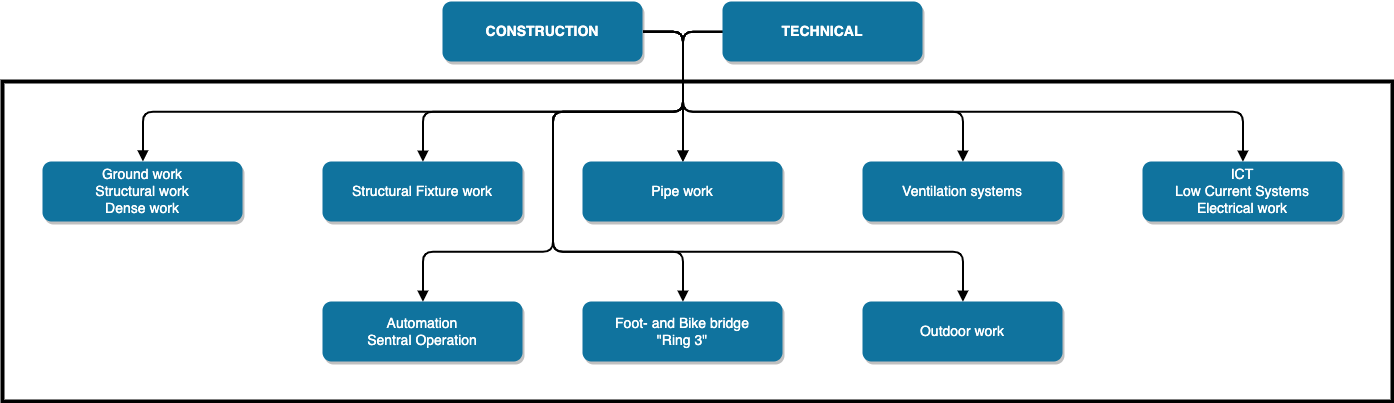
\includegraphics[width=\textwidth]{fig/LVB_contracts.png}
    \caption{Contruction Contracts in the Life Science Building Projects, each managed by either the construction- or technical project manager. (Statsbygg)}
    \label{fig:project_contracts}
\end{figure}

\subsubsection*{The Lean Strategy}
The Lean Strategy applied in the LSB-project is tailor-made from experience from both the Domus Medica- and BAAD-project. Two Lean strategies are applied in the LSB-project: 

\begin{enumerate}
    \item \textbf{Lean Design:} A method conserning design management and design coordination to ensure that the progress and knowledge sharing, in the Design Phase, is as good as possiblble.
    \item \textbf{Lean Construction:} A method conserning the scheduling
    of tasks and the availability of skills and materials to ensure that the work progresses as smoothly as possiblble during the construction.
\end{enumerate}

Different from the traditional design phase described in section \nameref{sec:CI_context}, the LSB-project made use of an iterative method. The \textit{Lean Design}-method has been developed by Statsbygg, after designing the Domus Medica and BAAD projects. In all projects utilizing Lean as their project methodology, the LSB-project also iterates over a product. The product, in this context, is the BIM model. Moreover, the project makes use of Level of Development (LOD), mentioned in the \ref{sec:lean_construction} section, where each iteration, named sequence, has the intention of getting the BIM model more mature. Also, based on the Contract strategy, the result of this process is not procurement, but the final product ready for implementation - hopefully without bugs. 

A problem with the traditional design phase was evaluating the overwhelming amount of documentation at the end of the phase. Furthermore, it is an argument in the Agile manifesto. Having sequences, the Lean Design method, therefore, made it easier having control over all interdisciplinary correlations. In LSB-project, these sequences last up to two weeks. In every sequence, the project leaders are assigned a set of packages. Ending the sequence, the project leaders need to deliver on the packages assigned. This way, the project can identify tasks that are, or can be, risks for the project. Every week in the designing the project starts with a cermony named blackboard-meeting. In this meeting all project leaders, project managers, and responsible goes through the packages and deliveries due to that meeting, or the status if not the end of a sequence. The project chair the meeting, while the rest need to the status of the their area of responsibility. 

The Detail project started with a two-week planning session, which made all trailing package-planning possible. The session resulted in the process map. The process map includes four levels of tasks, illustrated in figure \ref{fig:Milestones-Keypoints-Deliveries-Actions}: (1) the Milestones: A significant planned completion of a part of the project, e.g., steering document approved; (2) Key Points: Key Points is less significant, and with a shorter time frame than milestones, but in the same way an indication of completion; (3) Deliveries: A Key Points consists of several deliveries, e.g., finishing a room or design of a floor; and (4) Actions: Actions is everything needed to be done to complete a Delivery. 

\begin{figure}
    \centering
    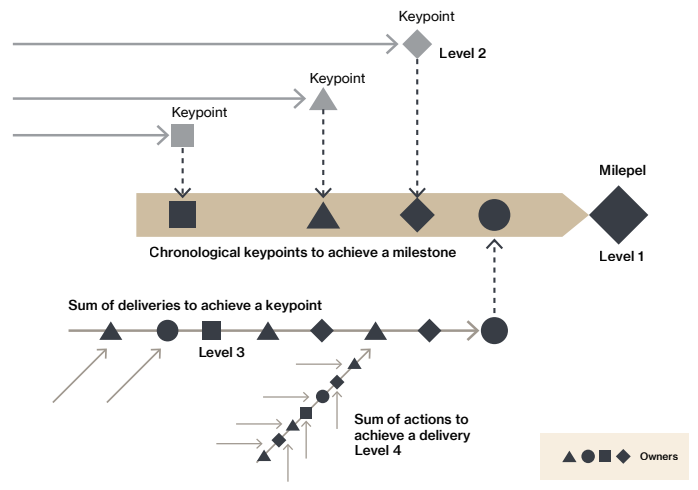
\includegraphics[width=0.8\textwidth]{fig/LSB_task_levels.png}
    \caption{Contruction Contracts in the Life Science Building Projects, each managed by either the construction- or technical project manager.}
    \label{fig:Milestones-Keypoints-Deliveries-Actions}
\end{figure}

Both the Lean Construction, described in section \ref{sec:lean_construction}, and Lean Design, make use of large planing tables. These can look like the old roadmaps used when planning the coding in Waterfall. Depending on how one makes use of the plans, the result of such planes is that they often than not end up wrong. Therefore, as Sutherland points out in his book \cite{sutherland}, the plan is not the final solution, the plan is what is needed, and adapt thereafter. Though, in this case it seems like the time was well spent giving the project leaders valuable insight into the project. Not spendig too much time planning ahed. 

\subsubsection*{The Strategy of Systematic Completion}
As described in section \ref{sec:CI_context}, the construction process ends with the Realization phase. It is after this phase, the project, or building in our case, is tested. If tests run smoothly and the owner approves the construction, the building handover occurs. The mission of testing is to verify that the final product meets the initial requirements and specifications defined. A typical case, when conducting these sorts of tests, is discovering errors. Problems getting wors when there is no control of these errors. If the final construction has too many errors, the owner can decide not to take over the building. Consequently, the project fails to deliver on schedule. Sadly, this happens quite often.

Managing this issue, the LSB-managers has developed a method, checking the systems, functions, and geometry of the construction. The method is named \textit{Systematic Completion} (SC). Throughout the project, SC is conducted, reducing the risk of not deliver the final project. SC follows the LOD-version, which makes for successful completion, with the correct level of quality, at the right time.

\subsubsection*{The Digitalization Strategy}
The Digitalization strategy is, both important in itself, but also supportive in regards to the other strategies. The project using a digital 3D visualization of the building as the product, driving the Lean Design method. Revit, the BIM modeling tool, is, in many ways, the core of the project, supported by dRofus, which is the room database. Prominent in the strategy is connecting all software used in the project and making all entrepreneurs use the same. Hopefully, one can trace the socket implemented in a room, by an electrician, through the drawings given, back to the BIM-model, and the dRofus database, where it was first planned. The resulting system can later be used by janitors, running the building, to identify errors in the system.  Figure \ref{fig:LSB_systems} visualize the connected systems in the project.

\begin{figure}
    \centering
    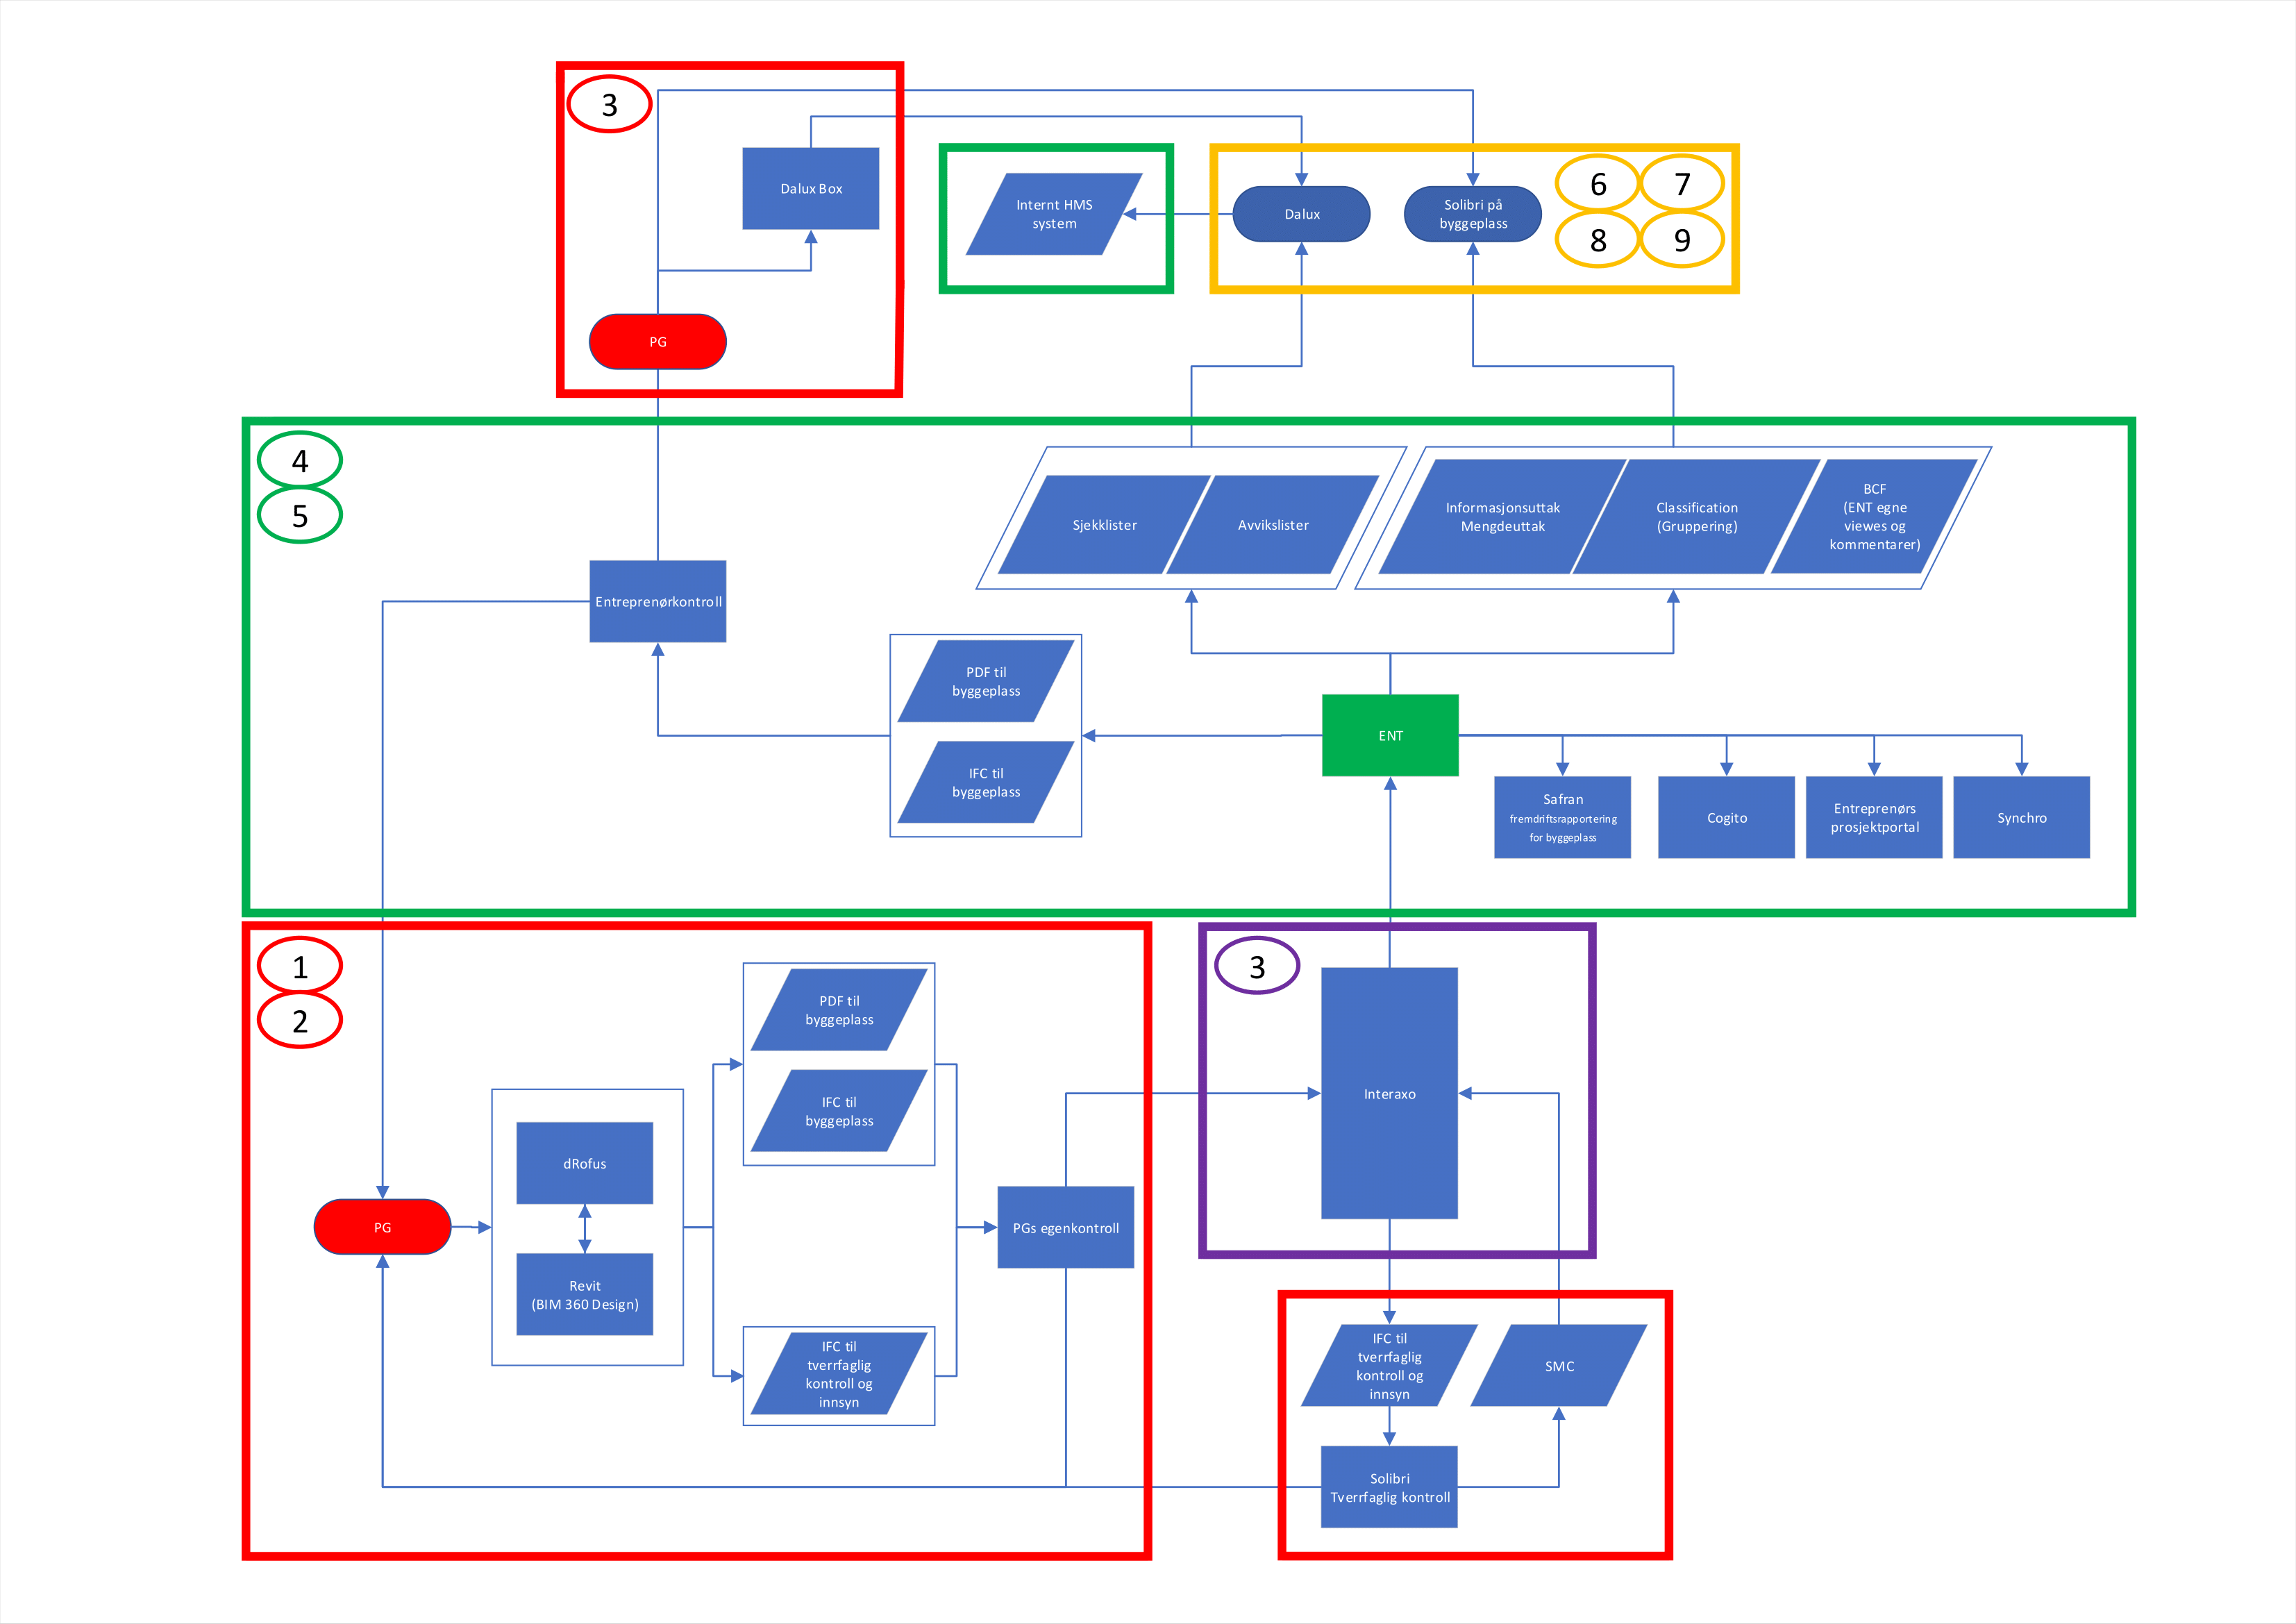
\includegraphics[width=\textwidth]{fig/LVB_system-arkitektur.png}
    \caption{Overview over the system architecture used in the Life Science building project. Outlines representes the actors using the systems, by color: (red) Project group, (green) Entrepreneurs, (yellow) HSE, and (blue) cloud service sharing documents}
    \label{fig:LSB_systems}
\end{figure}

A significant part of the digitalization, and unique for the LSB-project, is the deployment of the Cogito Project-system. Cogito is a tool used to visualize the planning done in the design phase, supporting the Lean Design method. The tool are beeing used tracking actions, deliveries, and Key points and milestones, who is responsible. Furthermore, calculate Planned Percent Completed (PPC), which is an excellent way of identifying delays. The project is planning to use Cogito tracking both the design- and the implementation phase of the project.

The project utilizes, added to Cogito, several other software supporting Agile project management and cooperation. Under following a list of the most crucial software, concerning Agile and collaboration. 


\begin{itemize}
    \item {\bf Revit:} BIM modeling tool, used in the design and construction of the project. Revit is a local software for every modeler, architect, and worker modelling. The software is developed by Autodesk, which also developed the much popular Autcad; a computer aided design tool for architects, engineers and proffesionals in the construction business. Creates drawings in 2D and 3D. When finished modeleing the modeler has to export what is done so available for the rest of the project. The exportation from every dicipline is put together in the common model, once a week.
    \item {\bf dRofus:} Software supporting BIM. Whats defined in dRofus is known as the truth if there is a mismatch between BIM and dRofus. The software is used as the database for the BIM model and used in the planning of every room. Furthermore, the data stored in dRofus is being used in the procurement of systems and objects to the project. Every element in the project is given a specific id; a TFM number. This number is later used in implementation, when a object is placed in the building it recieves a corresponding TFM-tag. Later, when the building is running a janitor can fix an object and know exactly what type it is based on the object's TFM.
    \item {\bf Cogito:} Visualization of ongoing and planned packages, in both the design phase and construction phase of the project. The project director and other managers of the LSB-project have formed the Cogito project, through experiance and some are also invested in the tool. Though, has to take thus are invested in the project. The idea of the tool came from the needs encountered in previous projects \cite{lean_i_praksis}. The tool is a supplement for a Lean Design and Construction process, specialy shapet for the construction business. The software is developed by a company named Tasctrl, and was only partly finished when introduced to the project. 
    \item {\bf Interaxo:} Cloud service for documents. Servicing onboarding, breach handling, and offboarding. Ineraxo is a platform gathering almost all the documents needed in a construction project. The high demand for documentation is simpler using this tool. After finishing a task in Cogito the final documentation ends up in Interaxo. Often there is a link to Interaxo in the preluminary field in Cogito.
    \item {\bf Blink:} Communication tool and intranet for the project. Using BLink, interactions can happen rapid and informally without booking meetings and writing extensive emails. Moreover, Blink has wide variety of features like News feed, documentation, messaging and in depth analysis of the workforce. Though, the project main requirement was the newsfeed, the software was chosen due to its confidentiality and security policies. Other services like this are Facebook Business manager and Atlassian Confluence. 
    \item { \bf Solibri:} Bringing all models from all dicipline in to one view. Gives all actors access to the model, and offers advanced checking and quality assurence, like collision tests. The tool give everyone involved the possibility to collaborate and solve any found issues. A user can view the model and minimize the model as needed. 
    \item { \bf BIM 360:} BIM 360 brings together all aspects of construction in BIM into one platform. Autodesk develops the product, thus integrates with Revit. The software aims to remove the silo structure, often appearing in a project including different themes and disciplines. Offering a shared platform for them to see, collaborate, and develop the Revit model online. Moreover, set up teams, restrictions, and team workspaces. Also, supporting LOD throughout the model. The project has procured BIM 360 Design, hereby refered to as BIM 360, which is one of seven products offered in the BIM 360 sphere.
   \end{itemize}

\subsubsection*{The Logistics Strategy}
Last, the Logistics Strategy. When coordinating a large number of people and paraphernalia, having control is a major challenge. In the LSB-project, there will be up to 800 people and equipment worth over 1 million NOK.  These numbers argue for the logistics strategy. The strategy involves planning for goods arriving the lot, as well as where one should tossing the garbage. Considered in this strategy is also removing packaging before arriving the lot, where the goods should arrive, securing the most effective utilization of construction workers. Should the project construct a cantina, so the workers do not have to walk to the nearest McDonald's or grocery store when having lunch? Furthermore, alining workers, equipment, and goods needed to support the train in the Lean Construction strategy. This strategy could be a significant impact when considering the overall labor productivity of the project. 


\subsection{Project management in the Life Science Building-project}
To manage a project, this significant, the constructing organization makes use of several different management approaches. One can divide the project management into two levels: (1) process management: The support of the process and how the teams are working together, and in what order; and (2) implementation management or method management: The management of design and implementation of the final product. The organization structure used in the project supports the two levels of project management. The first of the two, process management, is using customized phase-based process management, inspired by agile thinking. Second, implementation management utilizing the above strategies. 

The construction project organization structure is, as seen in figure \ref{fig:project_structure}. Starting at the top, in charge of the project, is the project director (PD), supported by the assisting project director (APD). The board, seen on the right, consists of four managers, each responsible for different strategies of the project. On the left HSE and project support, which is responsible for i.a. Communication, economics, progress. Beneath the four divisions in the project, where design is responsible for process and management. Paraphernalia is responsible for equipment in the final building. Construction and Technical are two divisions responsible for the eight contracts. In each of the division a Project Leader (PL) is responsible. The PL in Construction and Technical the PLs are responsible for the projects concerning their contracts.

\begin{figure}
    \centering
    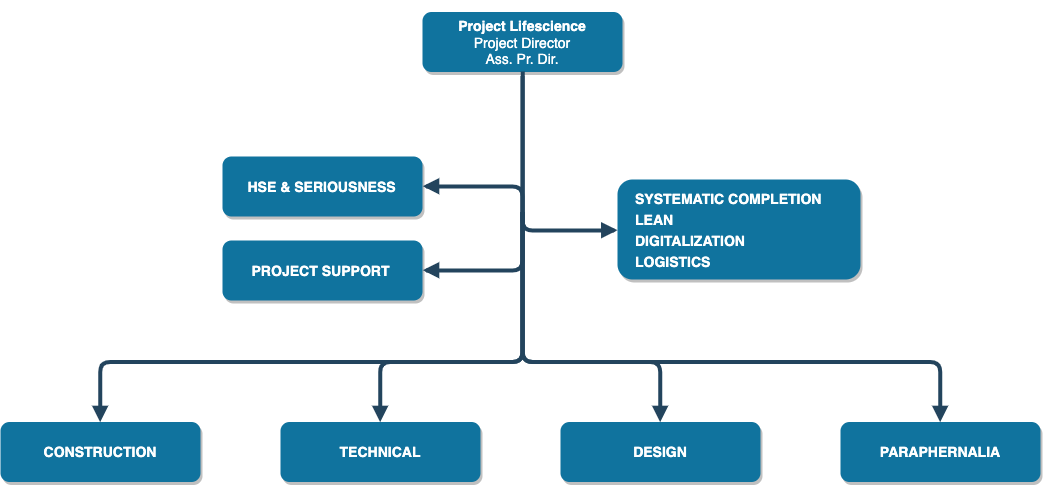
\includegraphics[width=\textwidth]{fig/lvb_diagram.png}
    \caption{Organizational structure in the Life Science Building Project.}
    \label{fig:project_structure}
\end{figure}

\section{Results of the case study}
The research, described in chapter \ref{chp:method}, resulted in three themes. These themes were selected based on their significance toward the research question. This next section introduces these themes, with general observations, such as recurring points of agreement and disagreement, trends, and patterns. 

The themes chosen are as follows: (1) \nameref{sec:unmitigated}: The project uses a lot of digital tools. Some overlap in their function and different actors in the project use them differently; (2) \nameref{sec:lack_of_knowledge}: The project makes use of newer, and self-made, methodology and techniques, in which require knowledge and understanding.

\subsection{Overlapping Software Functionality and Software Usage} \label{sec:unmitigated}
The project makes use of a lot of digital tools, some of them mentioned in section \ref{sec:case-intro}. In addition to all the tools that are decided by the governing organization, every contractor or team can choose to introduce new tools aiding their work. This makes for an extensive set of digital tools utilized in the project. When considering that a considerable amount of workers are only working part-time on the project, one can imagine the difficulty of getting an overview. Furthermore, throughout the project, the tools differ in use; Causing a competition in which tools to use.

By the law, a project can not dictate which tools the modelers, architects, and workers use to do their work due to competition rules. For example, when contracting a contractor doing the modeling, the governing organization can only decide on the resulting file-type in which the contractor is to enrich the model. Thus, giving a variety of tools throughout the project. Even though the governing organization can not decide all the tools, some are, and the project itself contracts these. Examples of tools chosen, and contracted, by the governing organization are project management tools for collaboration, documentation, and overview, such as Cogito, Interaxo, Blink, Solibri, and BIM 360.

A project like LSB includes a variety of different disciplines, and with that follows a wide variety of working habits. Still, the PLs need to utilize some structure to control and monitor the project and project progress. Thus, implement Cogito, Interaxo, Blink aiding this control. The idea is for everyone to use these tools, giving traceability and transparency to the PLs. This full use is not so much the case in the project. Several workers were reporting they do not or seldom use these tools. Especially Blink, where almost everyone reported they did not use it, or see it as no necessity. 

Blink is later proven critical because the project is posting all information regarding the measures taken on the Covid-19 outbreak.

Moreover, a tool giving a direct overview of the project progress is Cogito.  Everyone should have access to Cogito, giving them access to what is going on in the project and what is due the next days and weeks. It is, therefore, striking the disagreement about the tool. Some have chosen not to use it within their discipline. While others use it in meetings, showing the progress and the future deadlines, for the team to deliver. The method of use is also different in various disciplines and managers. 

This span in adaptation is an example of how new software is difficult to inject into an organization. Let alone when the software supports a new way of working. Following this new way of working, this tool is leading others to choose not to integrate this tool with the team.

Several teams have been reporting using other task management tools and different tools within the team. Some of these tools offer services, which the tools set by the governing organization does not support. Though, some of them contribute to overlapping functionalities. Thus, the overlap could result in double-entry or not using the common tool, which will hamper the transparency. The implementation of other tools will be reviewed later in this section. 

The different use of tools such as Cogito may have roots in the different understanding and use of the tool. How the project uses Cogito is based on Lean Construction and Lean Design. Thus every package has some predefined fields of input, including deadline, prerequisites, title, and description. The project does not have a standard way of filling these inputs. Thus, every team and package reporter operates differently throughout the project. Especially how to write package descriptions and prerequisites wearies a lot. 
One engineering manager reports using previous packages as a baseline for new packages. Thus, giving consistency to the rest of the team and other disciplines reading the packages. One can argue a lack of knowledge, as of the next section, but in this case, there is no standard way defined in the methodology on how to write package descriptions. Moreover, how to set deadlines, and notifying others about it, is not defined in common ground. Thus, leading to surprises and late deliveries. 

\begin{quote}
    \textit{"I have been part of several themes. The same tools are not used."}
    \\ - Associate, about different tools applied
\end{quote}

Table \ref{tab:software-map} illustrate the overlap in software utilization. The list of different task management tools and issue trackers, illustrate the variety of different tools available. The project only dictates the use of Cogito in interdisciplinary and Lean Design process tasks. Thus, the different disciplines and teams are free to use the task management and issue tracking tool of choice to conduct the discipline-specific assignments. Every consultant is bound only to the small set of software dictated by the manager. Hereafter they are free to use every tool needed to fulfill their task. Thus, in a project with a large number of firms, the number of different tools will increase. The people suffering in this environment are the engineers working in different teams. Hence, the comment about different tools applied. 

Some of the tools implemented by the owner have much functionality, which overlaps with other software applied. The idea with the software applied is to solve a purpose; Cogito is for package follow-up, Interaxo for documentation, BIM 360 is for BIM-collaboration in real-time, Solibri is to look at the model, Revit is for modeling, and e-mail is for communication. All these software offers a lot more actions then described here. Some of these actions overlap with actions to be done in other tools. Thus, the project has to define which tools to do specified assignments: this way, PLs, and management can follow-up tasks, teams, and packages, without having to seek for it. 

An example is in Cogito, a project member reports an action, and the responsible starts discussing this package with a contractor over e-mail, rather than using the discussion panel in Cogito. Thus, the transparency is lost, and going back to see how one solved the package could be challenging because of where the discussion took place is not known. Also, different parts of the project use different tools for the same process. Where one theme-group does issue management in 3D modeling in BIM 360 Design, others tend to use BIMcollab. While project management does not care how modelers work, this could be difficult for an engineer working on several theme-groups and teams throughout the project.

All these different tools make for a competition against which tool to use, between the different actors. Moreover, several tools do not just overlap in functionality, but one actually can replace the other. 

What causes all these different software to be deployed, one may want aks. Often the answer is as simple as what came first. In the case of BIMcollab versus BIM 360, that is the case. Before procuring BIM 360, several teams and consultants used BIMcollab. BIM 360 was recently procured when the interviews took place, early February. Hence, the comment on going from BIMcollab to BIM 360. Over time the issues will change from being stored in BIMcollab, but for now, they have to face using two separate tools. As one can see in table \ref{tab:software-map} BIM 360 and BIMcollab offers the same functionality for the project.

Different participants report using Microsoft Teams (Teams). Teams offer a wast variety of features, from direct messaging (chat) to task management and video chat, as seen in table \ref{tab:software-map}. Here, prior experience is the reason for use. Using teams makes for overlap with different predefined tools, giving either double reporting, using both tools, or using the wrong tool, not using the project tool. One can argue that Teams overlap with both Blink and Cogito. Blink supply the chat service. Moreover, Cogito is the primary task management tool in the project; thus, it works in smaller team management as well, which will eventually result in transparency for both the team and the rest of the project. A participant even proposed using Teams for much more than an issue manager, removing Cogito as a hole. Arguing Teams can visualize the project in the same way or better than Cogito.

Prior experience is also the reason for the different Modeling tools applied. The majority is using Revit, but some stick to Civil 3D. The modeling tool is for the modeler how the hammer is for a carpenter. Therefore forcing someone using a specific tool is foolish. As long as the different actors can cooperate, the tools they use are negligible. Hence, all overlap is not foolish.

Furthermore, in Interaxo, the documentation tool, one can see a different way of use between various teams. So much that several project members do not know of the structure set by the project management. 

Using these tools is a part of the process set by project management, and one can not blame the tools themself. The project has defined a process of onboarding new project members. Though, it seems like several new members have not received this. Part of this process is a course in Lean, as well as how to use the applied tools. Onboarding will give an overview of the tools applied, also why the project is using them. Moreover, the underlying methodology and processes are to be understood before utilizing the tools supporting them. Hence, the next section is discussing the lack of fundamental knowledge.

% Please add the following required packages to your document preamble:
% \usepackage{booktabs}
% \usepackage{longtable}
% Note: It may be necessary to compile the document several times to get a multi-page table to line up properly
\begin{longtable}{@{}lp{0.25\textwidth}p{0.45\textwidth}}
    \toprule
    \textbf{Software} &
      \textbf{Function} &
      \textbf{Comment} \\* \midrule
    \endhead
    %
    Cogito &
      \begin{tabular}[c]{p{0.25\textwidth}}Task management\\ Process management\\ Risk management\end{tabular} &
      \begin{tabular}[c]{p{0.45\textwidth}}"Provisionally we have not used Cogito in our team."\\ - Progress Planner, about Cogito \\ 
        \\ "Often, there is suddenly a package in Cogito. There are no notifications in cogito, which indicates that a package is given to you. If it is, it is not so intuitive, as it is now." \\ – Discipline Leader, about notifications in Cogito \\ 
        \\"...there is a notification functionality, but that does not work optimally."\\
      – Engineering Manager, about notifications in Cogito \\ 
      \\ "Cogito is a project overview-tool, but the presentation it gives is not always apparent" 
      \\ - Project Leader, about overview in Cogito \\
      \\ "After finishing my tasks, I am checking Cogito for something to do. Although it should have been the other way around." \\
    – Associate, about Cogito \\
      \\ "...as well as being a great way of visualizing the plan for the rest of the team." \\
     - Engineering Manager, about using Cogito in meetings \\ \end{tabular}
     \\* \midrule
    SharePoint &
      \begin{tabular}[c]{p{0.25\textwidth}} Task management\\ Information Sharing\\ Document Collaboration \end{tabular} & 
      \begin{tabular}[c]{p{0.45\textwidth}} "I wish we were using SharePoint for everything in the project ... Instead of using Cogito" \\ - BIM Coordinator \\ \end{tabular}
       \\* \midrule
    Microsoft Teams &
      \begin{tabular}[c]{p{0.25\textwidth}}Task management\\ Direct messaging (chat)\\ Video chat\\ \\ Calendar\end{tabular} & 
      \begin{tabular}[c]{p{0.45\textwidth}}"We have used e-mail and Teams for internal tasks, but we do not put these into Cogito."\\ - Discipline Leader, about Cogito \end{tabular}
       \\* \midrule
    Email &
      \begin{tabular}[c]{p{0.25\textwidth}}Direct messaging\\ Information sharing\end{tabular} &
      \begin{tabular}[c]{p{0.45\textwidth}}"Using email is very easy, I think"\\ - Associate, about using email\\ \\ "Unfortunately, a lot of communication takes place over email. That is a cumbersome process, I think."\\ - BIM Coordinator, about using email\\ 
        \\ "I am struggling to keep up with all the emails." – Ass. Project Group Leader, about using email\\
        \\ "It is not unmitigated where to communicate. We have email(...), then we have Interaxo (...). Lately, BIM 360 has been introduced."\\ - Associate, on communication. \\
     \end{tabular} \\* \midrule
    Skype &
      \begin{tabular}[c]{p{0.25\textwidth}}Video Chat\\ Direct Messaging\end{tabular} &
      \begin{tabular}[c]{p{0.45\textwidth}}"We use Skype, and when they are at the office, we take it here."\\ - Discipline Leader, about using Skype\end{tabular} \\* \midrule
    Blink &
      Information sharing &
      \begin{tabular}[c]{p{0.45\textwidth}}"Have not received an invitation, but I have heard about it. That is the social network?"\\ - Associate, about Blink\\ \\ "Everyone in the project has Blink, but I think it is quite uninteresting. I see it more as a social thing, which could be nice."\\ - Discipline Leader, about Blink\end{tabular} \\* \midrule
    Interaxo &
      Documentation &
      \begin{tabular}[c]{p{0.45\textwidth}}"In Interaxo, the same structure is not applied in all directories."\\ - Associate, about Interaxo\end{tabular} \\* \midrule
    Solibri &
      \begin{tabular}[c]{p{0.25\textwidth}}Model viewing\\ Model extraction\end{tabular} &
       \\* \midrule
    Revit &
    BIM modeling &
        \begin{tabular}[c]{p{0.45\textwidth}}"It is stated that in this project Revit is used. Revit is not as suitable for parts of our discipline's work, hence we use Civil 3D"\\ - Discipline Leader, about modeling tools\end{tabular} \\
    AutoCAD Civil 3D &
        BIM modeling &
    \\* \midrule
    BIMcollab &
      \begin{tabular}[c]{p{0.25\textwidth}}BIM communication\\ Issue tracker\\ Collision control\\ Model viewing\end{tabular} &
      \begin{tabular}[c]{p{0.45\textwidth}}"We used BIMcollab, before BIM 360. We have spent time and money teaching people using BIMcollab. Let alone created all the issues. We can say that we are to use BIM 360 with all its features, but that is large and difficult task, hard to complete. Thus, BIM 360 will be used, but not all the features."\\ - BIM Manager, about switching to BIM 360\end{tabular} \\
    BIM 360 Design &
      \begin{tabular}[c]{p{0.25\textwidth}}BIM communication\\ Issue tracker\\ Collision control\\ Model viewing\end{tabular} &
       \\* 
     \bottomrule
    \caption{Software map. Overview of different functions, coherent tools used, and quotes from project members.}
    \label{tab:software-map}\\
\end{longtable}

\subsection{Lack of Fundamental Methodological Knowledge} \label{sec:lack_of_knowledge}
To construct a building like LVB is, as we have seen, a complicated project, to complete the task of constructing this building depends on ingenuity, a good process, and solid management keeping everything in place. Moreover, one needs a whole lot of people to perform and cooperate. The people collected for the LSB-project are hired because of their specialty in their discipline. Some are the best Norway has to offer in terms of expertise. That does not mean they have worked in a project this extensive or complex as the LVB-project. Perhaps they are not familiar with the process applied in the project, namely Lean Construction, Lean design, and Systematic Completion. Thus, project workers, both experienced and less experienced, can feel a lack of understanding, ignorance, or possibly a shortage of knowledge. 

Lean heavily influences the LSB-project. Therefore, an introduction to Lean is mandatory in the project's onboarding process. As mentioned in the previous section, this onboarding is not fully accomplished. Hence, several project members lack knowledge of the process applied. 

It is clear to say that many of the project staff do not know Lean. Some have made their interpretations; others do know something, but not enough to understand the power it can provide adequately.  

\begin{quote}
    \textit{"I do have a Lean mindset, but I am not quite sure what Lean is."} \\
    - Associate, about Lean 
\end{quote}

Moreover, there is only one mentioning articulating using Lean Design in the design phase. Most of the interviewees seem not to understand that there is a Lean process present in the ongoaing phase. Moreover a process come constructing. 

\begin{quote}
    \textit{"That is something applicable come constructing, I have understood."} \\
    - Discipline leader, about Lean
\end{quote}

Furthermore, when not familiar with Lean, they will not recognize how and where Lean is applied.

\begin{quote}
    \textit{"We need to know how the strategies are to influence our actions."} \\
    - Engineering manager, about Lean
\end{quote}

A challenge when actors do not know the central method, the tools applied which are supporting the methodology is not understood. Hence,  many interviewees mentioned issues with Cogito. Several mentioned reports of missing overview. Due to the fact that Cogito is under development, one can imagine that some functionality is missing. Though,  what some actors are missing is the old Gantt-diagram, which the Lean Construction methodology does not support. Thus, the frustration against tools like Cogito often builds upon the lack of understanding. 

The fact that most of the actors interviewed do not recognize Lean Design in their description of the design process can point to other problems, also in the previous section. When not aligned with the same process or methodology, it is hard to cooperate and communicate. How one should assign tasks, write package descriptions, and do planning is often a part of a project methodology, and especially when considering agile project management. Therefore, the lack of knowledge considering Lean, and especially Lean design, is of a serious matter. It makes the basis of how the project is run, and therefore the tools applied and how to interact.

Added to Lean the project applies several other project management strategies, which, for some, could seem new, including Systematic Completion and Level of Detail/Level of Development (LOD).  

The LOD is, in the project, implemented somewhat in a unique approach. Usually, when talking about LOD, one consider the 3D-model; the BIM-model. The LOD variant applied in the LSB-project is known as MMI: Model Development Index. This approach, in itself, has shown to be difficult for some actors in the project. Especially defining the steps of the MMI-latter for every discipline, and what this means when writing package descriptions adding deliveries and actions to different parties. Actors articulate the suffering from the unawareness of LOD. 
\begin{quote}
    "Everything we do is done a new way. At times, it is unclear what the goal is. Thus, the planning of MMI has been difficult." \\
    – Engineering group leader, about MMI
\end{quote}
 
Furthermore, the project has implemented a sort of LOD in the rest of the project as well. Including both the digitalization and paraphernalia. Thus, project managers use this when deciding on procurement. Hence, some will say they spend too much time discussing the matter. The argument used by the owner is thus that they do not want to make the wrong decisions early on, and rather wait until their level of knowledge is acceptable. Then again, when the actors are not used to this way of working, it is difficult both in use and understanding.

The project suffers from a lack of knowledge. The project base the decisions and way of working on some pillars of methodology supported by the strategies. Though, it seems like there is a variety in the actors understanding of some these pillars. 
\cleardoublepage